\documentclass[10pt]{article}
\usepackage{commands}


\begin{document}
\begin{tcolorbox}
  \begin{center}
  \begin{Large}
    \textbf{PHYS 500 (Quantum Mechanics I) Notes} \\
    \vspace{5pt}
  \end{Large}
  \begin{large}
        Rio Weil \\
\vspace{5pt}
    \emph{This document was typeset on \today}
  \end{large}
  \end{center}
\end{tcolorbox}

\begin{center}
  \textbf{Introduction:}

  This is a set of lecture notes taken from UBC's PHYS 500 (Graduate Quantum Mechanics I) course, taught by Dr.\ Ariel Zhinitsky. The course covers Angular momentum and spin, electromagnetic interactions, Time-independent perturbation theory, the WKB approximation, Time-dependent perturbation theory, the adiabatic approximation, and scattering. If any errors are found in the notes, feel free to email me at \href{mailto:ryoheiweil@phas.ubc.ca}{ryoheiweil@phas.ubc.ca}.

\end{center}
\addtocontents{toc}{\protect\hypertarget{toc}{}}
\tableofcontents

\newpage
\section{Angular Momentum}

\subsection{Units}
We set $\hbar = 1$ for this course (natural units), unless we are doing a numerical estimate of some quantity.

\subsection{Angular Momentum - Definitions}
Angular momentum operators obey the commutation relations:
\begin{equation}
    [L_i, L_j] = i\e_{ijk}L_k.
\end{equation}
Where $\e_{ijk}$ is the Levi-Cicata symbol, defined as:
\begin{equation}
    \e_{ijk} = \begin{cases}
        +1 & ijk \text{ is an even permutation of 123}
        \\ -1 & ijk \text{ is an odd permutation of 123}
        \\ 0 & \text{otherwise}
    \end{cases}
\end{equation}
We also follow the Einstein summation convention, where repeated indices are implicitly summed over. We also define the raising/lowering operators:
\begin{equation}
    L_{\pm} = L_x \pm iL_y
\end{equation}
and the total angular momentum:
\begin{equation}\label{eq-Lsquared}
    \v{L}^2 = L_x^2 + L_y^2 + L_z^2.
\end{equation}
It can be easily verified that:
\begin{equation}
    [\v{L}^2, L_i] = 0
\end{equation}
and that:
\begin{equation}
    [L_z, L_+] = [L_z, L_x + iL_y] = +L_+
\end{equation}
\begin{equation}
    [L_z, L_-] = -L_-
\end{equation}
\begin{equation}
    [\v{L}^2, L_\pm] = 0
\end{equation}
Note that while $L_i$ are Hermitian operators (they are observables), the $L_\pm$ are not (this can be verified by the definition of the Hermitian conjugate). However this does not mean that it is not useful. Now, we ask, what is the physical meaning of:
\begin{equation}
    [\v{L}^2, L_z] = 0
\end{equation}
The answer is that we can know/measure $\v{L}^2$ and $L_z$ simultaneously. Next, what is the meaning of:
\begin{equation}
    [\v{L}^2, L_\pm] = 0
\end{equation}
This means that if we apply $L_{\pm}$ to an eigenstate of $\v{L}^2$, we do not change the eigenstate. Now, what is the physical meaning of:
\begin{equation}
    [L_z, L_+] = L_+?
\end{equation} 
It tells us that $L_+$ is a raising operator for $L_z$; it increments the eigenvalue of $L_z$. 

\subsection{Angular Momentum - Eigenvalues}
Let us now proceed with our construction. Consider the simultaneous eigenbasis of $\v{L}^2$ and $L_z$. Let us call the kets of this eigenbasis as $\ket{l, m}$. We want to solve the eigenvalue problem:
\begin{equation}
    \begin{split}
        \v{L}^2\ket{l, m} &= \lambda\ket{l, m}.
        \\ L_z\ket{l, m} &= m\ket{l, m}
    \end{split}  
\end{equation}
Let us back up for a moment; why can we define a simultaneous eigenbasis? Of course this follows from the fact that $\v{L}^2$ and $L_z$ commute:
\begin{equation}
    [\v{L}^2, L_z] = 0 \implies [\v{L}^2, L_z]\ket{l, m} = 0.
\end{equation}
Let us also check our physical interpretation of $L_+$. We know that $L_+\ket{l, m}$ should give us another eigenstate of $\v{L}^2$ and $L_z$ (which we can call $\ket{x}$), but to this end we calculate:
\begin{equation}
    [\v{L}^2, L_\pm] = 0 \implies [\v{L}^2, L_\pm]\ket{l, m} = 0.
\end{equation}
so we know that:
\begin{equation}
    \v{L}^2\ket{x} - \lambda\ket{x} = 0.
\end{equation}
Now, we know that $[L_z, L_+] = L_+$, so:
\begin{equation}
    [L_z, L_+]\ket{l, m} = L_+\ket{l, m}.
\end{equation}
Expanding the above, we have:
\begin{equation}
    L_z\ket{x} - m\ket{x} = \ket{x}.
\end{equation}
So rearranging we have:
\begin{equation}
    L_z\ket{x} = (m+1)\ket{x}
\end{equation}
And we can find an analogous result for $L_-$. We don't yet know how to normalize these states (we will do so later). But the above result is purely algebraic; no differential equations or spherical harmonics to be found. Let us continue and find the eigenvalues in an algebraic manner. If we recall the definition of $\v{L}^2$ in Eq. \eqref{eq-Lsquared}, we have:
\begin{equation}
    \v{L}^2 = L_z^2 + L_y^2 + L_x^2 = L_z^2 + (L_x + iL_y)(L_x - iL_y) + i(L_xL_y - L_yL_x). 
\end{equation}
Now using what we know of the angular momentum commutation relations and the raising/lowering operators:
\begin{equation}
    \v{L}^2 = L_z^2 + L_+L_- - L_z = L_z^2 + L_-L_+ + L_z
\end{equation}
Now, we consider applying the lowering operator $L_-$ many many times. We then get to a state with the lowest projection $m_{min}$. We then have that:
\begin{equation}
    L_-\ket{l, m_{min}} = 0.
\end{equation}
This arises from the fact that we cannot decrease $m$ further than the total angular momentum value (much in the same way that we cannot go below the ground state of the quantum harmonic oscillator). Analogously, we have:
\begin{equation}
    L_+\ket{l, m_{max}} = 0.
\end{equation}
Now, we apply $\v{L}^2$ to the minimum projection eigenstate. Then using the form of $\v{L}^2$ derived above, we have:
\begin{equation}
    \v{L}^2\ket{l, m_{min}} = (L_z^2 + L_+L_- - L_z)\ket{l, m_{min}}  = (L_z^2 - L_z)\ket{l, m_{min}} = (m^2_{min} - m_{min})\ket{l, m_{min}}
\end{equation}
and analogously:
\begin{equation}
    \v{L}^2\ket{l, m_{max}} = (L_z^2 + L_-L_+ + L_z)\ket{l, m_{max}}  = (L_z^2 + L_z)\ket{l, m_{max}} = (m^2_{max} + m_{max})\ket{l, m_{max}}.
\end{equation}
From this we obtain that:
\begin{equation}
    (m^2_{min} - m_{min}) = (m^2_{max} + m_{max})
\end{equation}
as the magnitude/eigenvalue of $\v{L}^2$ on the min/max projections should be the same. The above equation only has one nontrivial solution:
\begin{equation}
    m_{max} = -m_{min}.
\end{equation}
Now, we observe that we have an integer number of steps (as $L_+/L_-$ raise/lower by integers), so:
\begin{equation}
    m_{max} - m_{min} = N \in \NN
\end{equation}
And therefore:
\begin{equation}
    2m_{max} = N \implies m_{max} = \frac{N}{2}.
\end{equation}
That is to say that the eigenvalues of angular momentum can be integers or half-integers. We can conclude the eigenvalue relations:
\begin{equation}
    \v{L}^2\ket{l, m} = l(l+1)\ket{l, m}
\end{equation}
\begin{equation}
    L_z\ket{l, m} = m\ket{l, m}
\end{equation}
where $l$ or $m$ are either integers or half integers.

Now, we move onto the question of degeneracy. We have a $2l + 1$ degeneracy, where we count:
\begin{equation}
    m = -l, -l + 1, \ldots, 0, \ldots, l - 1, l.
\end{equation}
Now, we suppose we want to compute $\bra{l, m}L_x\ket{l, m}$. It turns out to be zero, but how do we show this? Physically, we can say that $L_x$ is completely uncorrelated with $L_z$ and so we should get zero. Mathematically we can use ladder operators:
\begin{equation}
    \bra{l, m}L_x\ket{l, m} = \bra{l, m}L_+ + L_-\ket{l, m} = \bra{l, m}\left(\ket{l, m+1} + \ket{l, m-1}\right) 0
\end{equation} 
where in the last relation we use that the $\ket{l, m}$ are orthogonal. Now we ask what about $\bra{l, m}L_x^2\ket{l, m}$? It is nonzero. We can calculate this by:
\begin{equation}
    \bra{l, m}L_x^2\ket{l, m} = \bra{l, m}\v{L}^2 - L_z^2 - L_y^2\ket{l, m}
\end{equation}
by symmetry we can conclude that $\bra{l, m}L_x^2\ket{l, m} =\bra{l, m}L_y^2\ket{l, m}$, and so:
\begin{equation}
    \bra{l, m}L_x^2\ket{l, m} = \frac{1}{2}\bra{l, m}(\v{L}^2 - L_z^2)\ket{l, m} = \frac{1}{2}\left[l(l+1) - m^2\right].
\end{equation}
\newpage
\section{Angular Momentum, Continued}
\subsection{Review of Lecture 1}
We start by reviewing the important points of last class. Using the commutation relations for $\v{L}^2, L_z, L_\pm$, we established that $L_\pm$ do not change the eigenvalue of $\v{L}^2$ when acting on an joint eigenstate of $\v{L}^2/L_z$, and we established the equations:
\begin{equation}
    \v{L}^2 = L_z^2 + L_{\pm}L_{\mp} \mp L_z.
\end{equation}
$\v{L}^2$ is the same for the highest and lowest states for $L_z$, and we established that $m_{max} = -m_{min}$. We found that the eigenvalues of $L_z$ jump in integer steps, and can take either integer or half-integer values. The main point is that we derived this purely algebraically (we did not solve Legendre polynomials). Note that 
\begin{equation}
    L_+\ket{l, m_{max}} = L_-\ket{l, m_{min}} = 0
\end{equation}
is equivalent to the boundary conditions when solving this problem in the differential equations approach. We found that:
\begin{equation}
    \bra{l, m}L_{\pm} \ket{l, m} = 0.
\end{equation}
by orthogonality, and using that $L_{x/y} = (L_+ \pm L_-)/2$ that:
\begin{equation}
    \bra{l, m}L_{x/y}\ket{l, m} = \bra{l, m}\frac{L_+ + L_-}{2}\ket{l, m} = 0.
\end{equation}


\subsection{Parity and Pseudovectors}
It is clear that:
\begin{equation}
    \bra{l, m}L_z\ket{l, n} = m.
\end{equation}
We now ask, what is the value of $\bra{l, m}Z\ket{l, m}$ and $\bra{l, m}X\ket{l, m}$? We find that:
\begin{equation}
    \bra{l, m}Z\ket{l, m} = \bra{l, m}X\ket{l, m} = 0
\end{equation}
as when we specify the angular momentum, we know nothing of the position.

How would we do this rigorously? We will come back to this when we do selection rules. For now, let us consider defining the parity operator $P$ that takes a vector $\v{v}$ and maps it to $-\v{v}$. So, each of the position operators get mapped to their negative (i.e. $P^\dagger XP= -X$). Using this in tandem with the fact that $\ket{l, m}$ are eigenvalues of parity (with eigenvalues $(-1)^l$, as we will discuss below), we could conclude that the above expectation values vanish, as:
\begin{equation}
    \bra{l, m} X \ket{l, m} = \bra{l, m}(-1)^l X (-1)^l \ket{l, m} = \bra{l, m}P^\dagger X P\ket{l, m} = \bra{l, m}(-X)\ket{l, m} = -\bra{l, m}X\ket{l, m}
\end{equation}
and comparing the first and last expressions we find that the expectation value is zero. However, we may then ask why does the expectation value of $L_z$ not vanish? This is because angular momentum (like torque and magnetic fields) are not vectors, but rather pseudovectors.

\subsection{Parity Spherical harmonics}
A last note about the eigenkets of angular momentum. In the position basis, we can write them as spherical harmonics:
\begin{equation}
    \ket{l, m} \cong Y_{l}^m(\theta, \phi).
\end{equation}
Consider a unit vector in 3d:
\begin{equation}
    \hat{n} = (n_x, n_y, n_z) = (\sin\theta\cos\phi, \sin\theta\sin\phi, \cos\theta).
\end{equation}
How do the spherical harmonics behave under $Y_l^m(\hat{n}) \to Y_l^m(-\hat{n})$ (in terms of angles, $\theta \to \pi - \theta, \phi \to \phi + \pi$) They transform as:
\begin{equation}
    Y_l^m(-\hat{n}) = (-1)^lY_{l}^m(\hat{n}).
\end{equation}
Let us look at a couple examples. $Y_0^0 \sim \frac{1}{\sqrt{4\pi}}$ so is unchanged under the flip of the vector. $Y_1^0 \sim \cos\theta$ so this maps to $\cos(-\theta) \to -\cos\theta$ under a flip of the vector. $Y_1^1 \sim \sin\theta e^{i\phi}$, so the $\sin\theta$ stays the same under interchange but $e^{i\phi}$ flips sign so it maps to $-Y_1^1$. 

Note this discussion is really trying to motivate the use of symmetry to skip doing computations; we don't have to compute integrals if we know the symmetry of the system.

Another example (returning to the above discussion of expectation values of position). Hopefully by now we would be convinced that:
\begin{equation}
    \bra{l, m}\v{R}\ket{l, m}  = 0.
\end{equation}
by the above arguments showing that $\ket{l, m}$ are eigenvalues of parity with eigenvalue $(-1)^l$. Now what about $\bra{l+1, m}\v{R}\ket{l, m}$? In this case it is \emph{nonzero} as the negative signs cancel when we consider the parity properties.

\subsection{Eigenvalues of Ladder Operators}
We know that the ladder operators follow the relation:
\begin{equation}
    L_+\ket{l, m} = c_+\ket{l, m+1}
\end{equation}
but we have yet to calculate $c_+$. Let us do this now. We consider acting $L_-$ on the dual of $\ket{l, m}$:
\begin{equation}
    \bra{l, m}L_- = c_+^*\bra{l, m+1}
\end{equation}
So therefore:
\begin{equation}
    \bra{l, m}L_-L_+\ket{l, m} = \abs{c_+}^2\braket{l, m+1}{l, m+1}
\end{equation}
so:
\begin{equation}
    \abs{c_+}^2\bra{l, m}\v{L}^2 - L_z^2 - L_z\ket{l, m} = l(l+1) - m^2 - m
\end{equation}
so we conclude:
\begin{equation}
    c_+ = \sqrt{l(l+1) - m(m+1)}
\end{equation}
and an analogous computation can be done to find $c_-$.

\subsection{Spin 1/2}
Because of the degeneracy of angular momentum ($2l+1$) derived via the Schrodinger equation, people expected to always see an odd number of lines when doing energy line experiments. But this turned out not to be true in experimental results; we require a new approach to the theory, developed by Pauli. We now thus explore spin 1/2 systems. For such systems, we have $s = 1/2$, where the spin operators follow the commutation relations:
\begin{equation}
    [S_i, S_j] = i\e_{ijk}S_k.
\end{equation}
Since there are $(2s+1)$ states, we have only two spin eigenstates:
\begin{equation}
    \ket{s = \frac{1}{2}, s_z = +\frac{1}{2}}, \ket{s = \frac{1}{2}, s_z = -\frac{1}{2}}
\end{equation}
Which obey:
\begin{equation}
    S_+\ket{s = \frac{1}{2}, s_z = +\frac{1}{2}} = 0,  S_-\ket{s = \frac{1}{2}, s_z = -\frac{1}{2}} = 0
\end{equation}
Given this, a natural notation for these states is:
\begin{equation}
    \ket{\uparrow} \coloneqq \ket{s = \frac{1}{2}, s_z = +\frac{1}{2}}, \ket{\downarrow} \coloneqq \ket{s = \frac{1}{2}, s_z = -\frac{1}{2}}
\end{equation}
So the above relations become (e.g.) $S_+\ket{\uparrow} = 0$. The total spin operator is given by:
\begin{equation}
    \v{S} \cong \frac{1}{2}\gv{\sigma}
\end{equation}
where $\gv{\sigma} = (\sigma_x, \sigma_y, \sigma_z)^T$, with the Pauli matrices given by:
\begin{equation}
    \sigma_x = \paulix, \sigma_y = \pauliy, \sigma_z = \pauliz.
\end{equation}
Note that there is no reference to coordinates whatsoever here; everything is purely algebraic. Now, what is the value of $\v{S}^2\ket{\uparrow}$? From the theory of angular momentum, we know that:
\begin{equation}
    \v{S}^2\ket{\uparrow} = s(s+1)\ket{\uparrow} = \frac{3}{4}\ket{\uparrow}.
\end{equation}
But let us derive this result using the matrix form of $\v{S}^2$. We can explicitly calculate to find that:
\begin{equation}
    \sigma_i^2 = \imatrix
\end{equation}
for each of the pauli matrices, so:
\begin{equation}
    \v{S}^2 \cong \frac{1}{4}(\sigma_x^2 + \sigma_y^2 + \sigma_z^2) = \frac{3}{4}\imatrix.
\end{equation}
So with the choice of representation that $\ket{\uparrow} \cong \m{1 \\ 0}$ and $\ket{\downarrow} \cong \m{0\\ 1}$, we find:
\begin{equation}
    \v{S}^2\ket{\uparrow} = \frac{3}{4}\ket{\uparrow},
\end{equation}
along with:
\begin{equation}
    S_z\ket{\uparrow} = \ket{\uparrow}.
\end{equation}
by looking at these matrix expressions. From now on, we will focus on spin-1/2 (though we will explore spin-1 in the homework). We will discuss the most general spin 1/2 state. It is given by:
\begin{equation}
    \ket{\chi} = c_+\ket{\uparrow} + c_-\ket{\downarrow}.
\end{equation}
In the spinor representation, it is given by:
\begin{equation}
    \chi = \m{c_+ \\ c_-}.
\end{equation}
How many real parameters are needed to specify the quantum state? Naively, we would say 4 (2 complex numbers). But it turns out to be only two. One parameter is reduced by the normalization condition:
\begin{equation}
    \abs{c_+}^2 + \abs{c_-}^2 = 1.
\end{equation}
We also have a reduction of one from the fact that the state is physically unchanged when multiplied by a global phase $\ket{\chi} \sim e^{i\phi}\ket{\chi}$; this comes from the fact that we can only measure probabilities in QM, and when we calculate these (using the Born rule, $p(i) = \bra{\psi}\Pi_i\ket{\psi}$ the global phase cancells out). An important distinction: \emph{relative} phases are observable (e.g. in neutron inferometry experiments), while global ones are not. So in the case of a single spin-1/2 particle, we can neglect the phase, but when we have multiple particles we cannot neglect relative phases.

\subsection{Magnetic Hamiltonians}
Consider the Hamiltonian:
\begin{equation}
    \H = -\gv{\mu} \cdot \v{B}.
\end{equation}
Where $\gv{\mu} = \gamma \gv{s}$. This $\gamma$ coefficient cannot be estimated by classical physics; a full calculation requires considering the Dirac field in QFT. But we can also evaluate it via experiment.

Next day, we will continue our discussion of this Hamiltonian and the evolution of spin states under it. We will also discuss Gauge invariance in the context of quantum mechanics.


\newpage
\section{Electron in EM field}
\subsection{Review of Spin}
We have the spin commutation algebra (identical to the angular momentum commutation algebra):
\begin{equation}
    [S_i, S_j] = i\e_{ijk}S_k.
\end{equation}
However, there is no way to represent the spin operators in spatial coordinate; we instead use matrices. Consider $s = 1/2$. Then we have $\v{S} = \frac{1}{2}\gv{\sigma}$, where $S_z$ has eigenstates $\ket{\uparrow} \cong \binom{1}{0}$ and $\ket{\downarrow} \cong \binom{0}{1}$. Any state can be expressed as a linear combination of these two:
\begin{equation}
    \chi = \frac{c_+}{\sqrt{\abs{c_+}^2 + \abs{c_-}^2}}\m{1\\0} + \frac{c_-}{\sqrt{\abs{c_+}^2 + \abs{c_-}^2}}\m{0\\1}.
\end{equation}

\subsection{Inner and Outer Products, Completeness}
We also have the inner product that gives us numbers:
\begin{equation}
    \braket{\uparrow}{\uparrow} = \m{1 & 0}\m{1\\0} = 1.
\end{equation}
Also note that outer products give us matrices:
\begin{equation}
    P_+ = \dyad{\uparrow}{\uparrow} \cong \m{1\\0}\m{1&0} = \m{1&0\\0&0}
\end{equation}
The above $P_\uparrow$ is a projector (that projects onto the spin-up subspace); as we have:
\begin{equation}
    P_\uparrow\ket{\uparrow} = \uparrow, P_+\ket{\downarrow} = 0.
\end{equation}
Note also the completeness relation:
\begin{equation}
    \dyad{\uparrow}{\uparrow} + \dyad{\downarrow}{\downarrow} = \II.
\end{equation}
As $\set{\ket{\uparrow}, \ket{\downarrow}}$ is an ONB for the spin-1/2 Hilbert space. When we have infinitely many states in an ONB, we have:
\begin{equation}
    \sum_{n=0}^\infty \dyad{n}{n} = \mathbb{I}, \quad \int \dyad{x}{x}dx = \mathbb{I}
\end{equation}
where the former is for a discrete ONB, the latter is for a continuous one (of course there are the caveats that $\ket{x}$ aren't really square-integrable states, but let us not worry about this). Now, a question: what is the $\dyad{\uparrow}{\downarrow}$? It is an operator that flips a down-spin to an up-spin:
\begin{equation}
    \dyad{\uparrow}{\downarrow} \cong \m{0&1\\0&0}
\end{equation}
Of course this is just the $S_+$ operator (it is not Hermitian, while $P_\uparrow$ is).

\subsection{Electron in Magnetic Field}
Consider the Hamiltonian:
\begin{equation}
    H = -\gv{\mu}\cdot \v{B}
\end{equation}
where $\gv{\mu} = \gamma\v{S}$ with $\gamma$ is a scalar known as the gyromagnetic ratio. It is equal to:
\begin{equation}
    \gamma = \frac{e\hbar}{2mc}2
\end{equation}
Note we've written $\gamma$ to include the $\hbar$ factor; usually $\hbar$ goes with $\v{S}$, but with our units convention, we prefer to write it this way. Note that if we calculate the gyromagnetic moment just by classical methods, we would just get $\frac{e}{2mc}$. The coefficient $2$ is the $g$-factor, which can be obtained by taking the nonrelativistic limit of the Dirac equation (we won't try to do this here); there is some hidden deep physics here we will leave for a different course.

Note that we have assumed that there is no orbital angular momentum for the electron (we only consider the intrinsic spin); a full treatment would take:
\begin{equation}
    \gv{\mu} = \frac{e\hbar}{2mc}\left(2\v{S} + \v{L}\right).
\end{equation}

\subsection{Electron in Magnetic Field in a single direction}
Now, we suppose a more specific scenario, where $\v{B}$ is aligned along the $z$-axis. We then have:
\begin{equation}
    H = -\gamma B_z\frac{1}{2}\pauliz.
\end{equation}
We have two easily solved eigenvalue equations:
\begin{equation}
    H\chi_+ = E_+\chi_+, H\chi_- = E_-\chi_-.
\end{equation}
Where $E_+ = -\frac{1}{2}\gamma B_z$ and $E_- = \frac{1}{2}\gamma B_z$. Now, a question; why is there a minus sign in $H$? The convention is such that the dipole moment wants to align with the magnetic field. 

Note that in our problem here, the $+$ denotes that we have a upwards projection (and a negative energy, as it is pointed along the field). Conversely, $-$ denotes that we have a downwards projection (and a positive energy). Of course, we know that:
\begin{equation}
    \chi_+ = \m{1\\0}, \chi_- = \m{0\\1}.
\end{equation}
and now everything is solved! We know the eigenvalues and eigenstates, so we have everything we need to determine the Schrodinger time evolution of the quantum state. We can say that:
\begin{equation}
    \chi(t) = \frac{c_+e^{-i\frac{E_+t}{\hbar}}}{\sqrt{\abs{c_+}^2 + \abs{c_-}^2}}\m{1\\0} + \frac{c_-e^{-i\frac{E_-t}{\hbar}}}{\sqrt{\abs{c_+}^2 + \abs{c_-}^2}}\m{0\\1}
\end{equation}

\subsection{Time-dependence of Observables}
For a most general spin-1/2 state, if we enforce the normalization condition of $\abs{c_+}^2 + \abs{c_-}^2 = 1$, then we can parameterize with just three parameters:
\begin{equation}\label{eq-chigeneral}
    \chi = e^{i\alpha}\m{\cos\frac{\theta}{2} \\ \sin\frac{\theta}{2}e^{-i\phi}}
\end{equation}
For now, let us discard the phases ($\alpha = \phi = 0$) and suppose that at $t = 0$ we have:
\begin{equation}\label{eq-chithetat0}
    \chi(t = 0) = \m{\cos\frac{\theta}{2} \\ \sin\frac{\theta}{2}}.
\end{equation}

Question: Let us compute:
\begin{equation}
    \avg{S_z}(t) = \bra{\chi(t)}S_z\ket{\chi(t)}.
\end{equation}
This turns out to be independent of time; let us see this in two ways. First, we can do the explicit calculation. $\chi(t)$ is given by:
\begin{equation}
    \chi(t) = \m{\cos\frac{\theta}{2} e^{i\omega t/2} \\ \sin\frac{\theta}{2} e^{-i\omega t/2}}
\end{equation}
Where $\omega$ is defined as the difference between the two frequencies. When we do the explicit computation, we find:
\begin{equation}
    \bra{\chi(t)}S_z\ket{\chi(t)} = \m{\cos\frac{\theta}{2} e^{-i\omega t/2}& \sin\frac{\theta}{2} e^{i\omega t/2}}\pauliz \m{\cos\frac{\theta}{2} e^{i\omega t/2} \\ \sin\frac{\theta}{2} e^{-i\omega t/2}} =  \frac{1}{2}\left(\cos^2\frac{\theta}{2} - \sin^2\frac{\theta}{2}\right) = \frac{1}{2}\cos\theta.
\end{equation}
If we do the same comnputation for $\avg{S_x}(t)$, we find that the time-dependence does not cancel out:
\begin{equation}
    \bra{\chi(t)}S_x\ket{\chi(t)} = \m{\cos\frac{\theta}{2} e^{-i\omega t/2}& \sin\frac{\theta}{2} e^{i\omega t/2}}\paulix \m{\cos\frac{\theta}{2} e^{i\omega t/2} \\ \sin\frac{\theta}{2} e^{-i\omega t/2}} =  \frac{1}{2}\sin\frac{\theta}{2}\cos\frac{\theta}{2}\left(e^{i\omega t} + e^{-i\omega t}\right) = \frac{1}{2}\sin\theta\cos(\omega t).
\end{equation}
We can picture this as the spin precessing at a fixed angle $\theta$ (fixed $z$-position).

\begin{figure}[htbp]
    \centering
    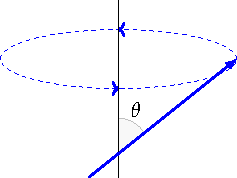
\includegraphics[]{Images/fig-spinprecess.pdf}

    \caption{When the initial spinor state $\chi(t = 0)$ is given by Eq. \eqref{eq-chithetat0} and evolves under a $z$-oriented magnetic field, the spin state can be visualized as precessing at fixed $\theta$ (the same $\theta$ as in the initial state). More technically, we could say that the spin state precesses at a fixed polar angle on the Bloch sphere; Note that the general spin state given in Eq. \eqref{eq-chigeneral} invites the visualization of a single spin-1/2 particle as a point on the unit sphere with polar coordinates $(\theta, \phi)$ (of course the global phase $\alpha$ is physically irrelevant).}
    \label{fig-spinprecess}
\end{figure}

However, there is a \emph{much} easier way to see why there is no time-dependence in the $S_z$ case, while there is a time-dependence in the $S_x$ case. The way to see this is that $[S_z, H] = 0$ ($S_z$ commutes with the Hamiltonian) so there is no time-dependence. Conversely, $S_x$ does not commute with the Hamiltonian, so we know that there is time dependence.

Let us discuss the simple case where:
\begin{equation}
    \chi(t = 0) = \frac{1}{\sqrt{2}}
    \m{1\\1}.
\end{equation}

Now, we want the probability of finding the spin to be in spin-up $P_\uparrow$ as a function of time. In this case, this will again be independent of time; a physical picture is that the spin precesses at a fixed angle, so the projection onto the $s_z$ axis does not change with time. A more concrete argument is that if we measure the probability of getting some outcome of an $S_z$ measurement, since $S_z$ commutes with $H$ then this probability should be independent of time. Let's see how this works out explicitly:
\begin{equation}
    \chi(t) = \frac{1}{\sqrt{2}}\m{1\\0}e^{i\omega t/2} + \frac{1}{\sqrt{2}}\m{0\\1}e^{-i\omega t/2}.
\end{equation}
By the Born rule we have::
\begin{equation}
    P_\uparrow = \abs{\braket{\uparrow}{\chi}}^2 = \frac{1}{2}
\end{equation}
which is time-independent. Let us now ask the probability of measuring $P_{+\xhat}$; how do we proceed? We start by finding the eigenstates of $S_x$:
\begin{equation}
    S_x \ket{\chi_{+\xhat}} = \lambda \ket{\chi_{+\xhat}} \cong \frac{1}{2}\sigma_x\chi_{+\xhat} = \lambda \chi_{+\xhat} \implies \chi_{+\xhat} = \frac{1}{\sqrt{2}}\m{1\\1}.
\end{equation}
We therefore can calculate:
\begin{equation}
    P_{+\xhat} = \abs{\frac{1}{\sqrt{2}}\m{1 & 1}\chi(t)}^2 = \abs{\frac{1}{\sqrt{2}}\m{1 & 1}\frac{1}{\sqrt{2}}\m{e^{i\omega t/2} \\ e^{-i\omega t/2}}}^2 = \abs{\frac{1}{2}\left(e^{i\omega t/2} + e^{-i\omega t/2}\right)}^2 = \frac{1}{2}\left(1 + \cos\omega t\right)
\end{equation}
Because the measurement is dichotomic, we can use completeness to find $P_{-\xhat}$:
\begin{equation}
    P_{-\xhat} = 1 - P_{+\xhat} = \frac{1}{2}\left(1 - \cos\omega t\right).
\end{equation}


\end{document}